\documentclass[a4paper]{article}\usepackage[]{graphicx}\usepackage[]{color}
%% maxwidth is the original width if it is less than linewidth
%% otherwise use linewidth (to make sure the graphics do not exceed the margin)
\makeatletter
\def\maxwidth{ %
  \ifdim\Gin@nat@width>\linewidth
    \linewidth
  \else
    \Gin@nat@width
  \fi
}
\makeatother

\definecolor{fgcolor}{rgb}{0.345, 0.345, 0.345}
\newcommand{\hlnum}[1]{\textcolor[rgb]{0.686,0.059,0.569}{#1}}%
\newcommand{\hlstr}[1]{\textcolor[rgb]{0.192,0.494,0.8}{#1}}%
\newcommand{\hlcom}[1]{\textcolor[rgb]{0.678,0.584,0.686}{\textit{#1}}}%
\newcommand{\hlopt}[1]{\textcolor[rgb]{0,0,0}{#1}}%
\newcommand{\hlstd}[1]{\textcolor[rgb]{0.345,0.345,0.345}{#1}}%
\newcommand{\hlkwa}[1]{\textcolor[rgb]{0.161,0.373,0.58}{\textbf{#1}}}%
\newcommand{\hlkwb}[1]{\textcolor[rgb]{0.69,0.353,0.396}{#1}}%
\newcommand{\hlkwc}[1]{\textcolor[rgb]{0.333,0.667,0.333}{#1}}%
\newcommand{\hlkwd}[1]{\textcolor[rgb]{0.737,0.353,0.396}{\textbf{#1}}}%
\let\hlipl\hlkwb

\usepackage{framed}
\makeatletter
\newenvironment{kframe}{%
 \def\at@end@of@kframe{}%
 \ifinner\ifhmode%
  \def\at@end@of@kframe{\end{minipage}}%
  \begin{minipage}{\columnwidth}%
 \fi\fi%
 \def\FrameCommand##1{\hskip\@totalleftmargin \hskip-\fboxsep
 \colorbox{shadecolor}{##1}\hskip-\fboxsep
     % There is no \\@totalrightmargin, so:
     \hskip-\linewidth \hskip-\@totalleftmargin \hskip\columnwidth}%
 \MakeFramed {\advance\hsize-\width
   \@totalleftmargin\z@ \linewidth\hsize
   \@setminipage}}%
 {\par\unskip\endMakeFramed%
 \at@end@of@kframe}
\makeatother

\definecolor{shadecolor}{rgb}{.97, .97, .97}
\definecolor{messagecolor}{rgb}{0, 0, 0}
\definecolor{warningcolor}{rgb}{1, 0, 1}
\definecolor{errorcolor}{rgb}{1, 0, 0}
\newenvironment{knitrout}{}{} % an empty environment to be redefined in TeX

\usepackage{alltt}

\usepackage[english]{babel}
\usepackage[utf8]{inputenc}
\usepackage{amsmath, amssymb, amsthm}
\usepackage{graphicx}
\usepackage[colorinlistoftodos]{todonotes}
\usepackage{float}
\usepackage[margin=0.75in]{geometry}

\newtheorem{thm}{Theorem}[section]
\newtheorem{defn}{Definition}[section]
\newtheorem{ex}{Example}[section]

\title{CIS 520 - Machine Learning Notes}
\author{Eric Oh - University of Pennsylvania}
\date{\today}
\IfFileExists{upquote.sty}{\usepackage{upquote}}{}
\begin{document}
\maketitle

\section{Local Learning}

The class of local learning methods seems less like learning and more like pure memorization - and in some ways it is. Main idea: given a new example $x$, find the most similar training example(s) and predict a similar output. We generally assume some measure of similarity or distance between examples and learn a \emph{local} method in a neighborhood of the new example. Consider the one dimensional regression problem:

\begin{figure}[H]
\centering
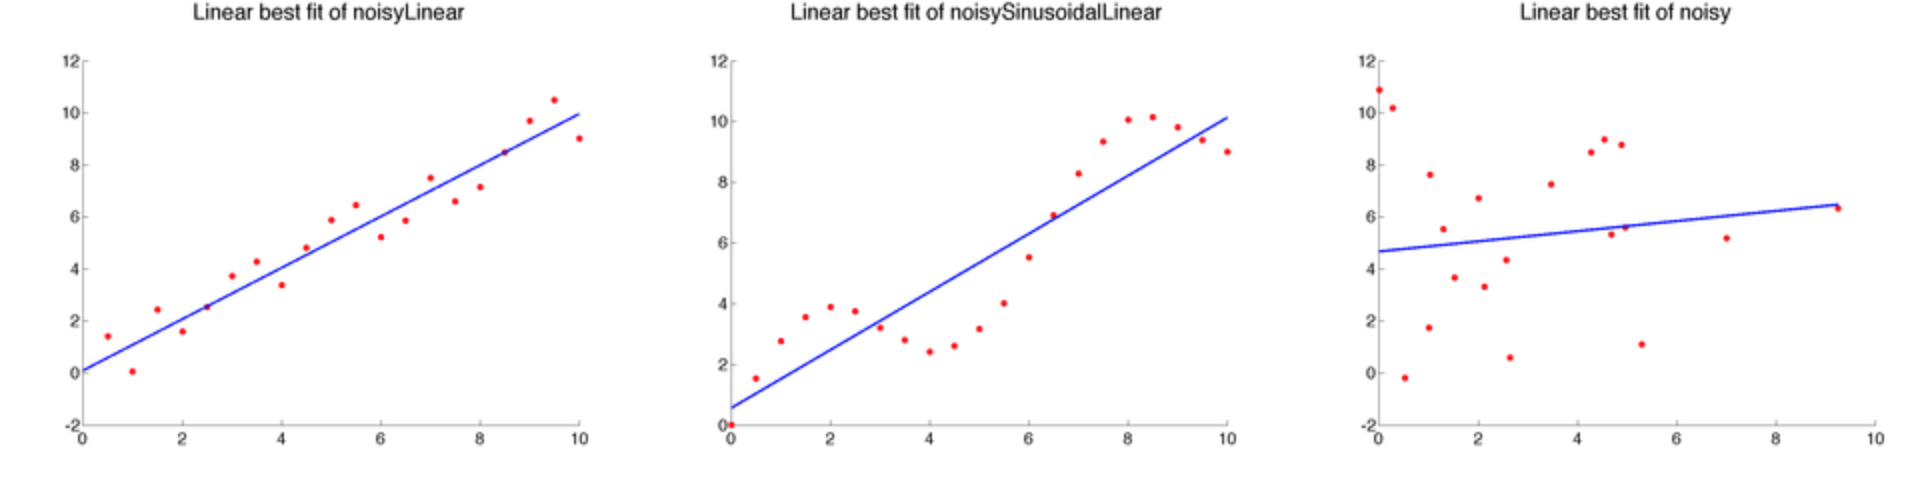
\includegraphics[width=6in]{badlinreg.png}
\caption{Clearly, linear model doesn't fit data well always}
\end{figure}

\subsection{Nearest Neighbor}

We could try adding higher-order polynomial terms or try a local method like nearest neighbors:

\begin{verbatim}
1 - Nearest Neighbor Algorithm 
  1. Given training data D={x_i,y_i}, distance function d(.,.), and input x
  2. Find j = arg min_i d(x,x_i) and return y_j
\end{verbatim}

Some examples of the above algorithm with $d(x,x_i)=|x-x_i|$ as x varies:

\begin{figure}[H]
\centering
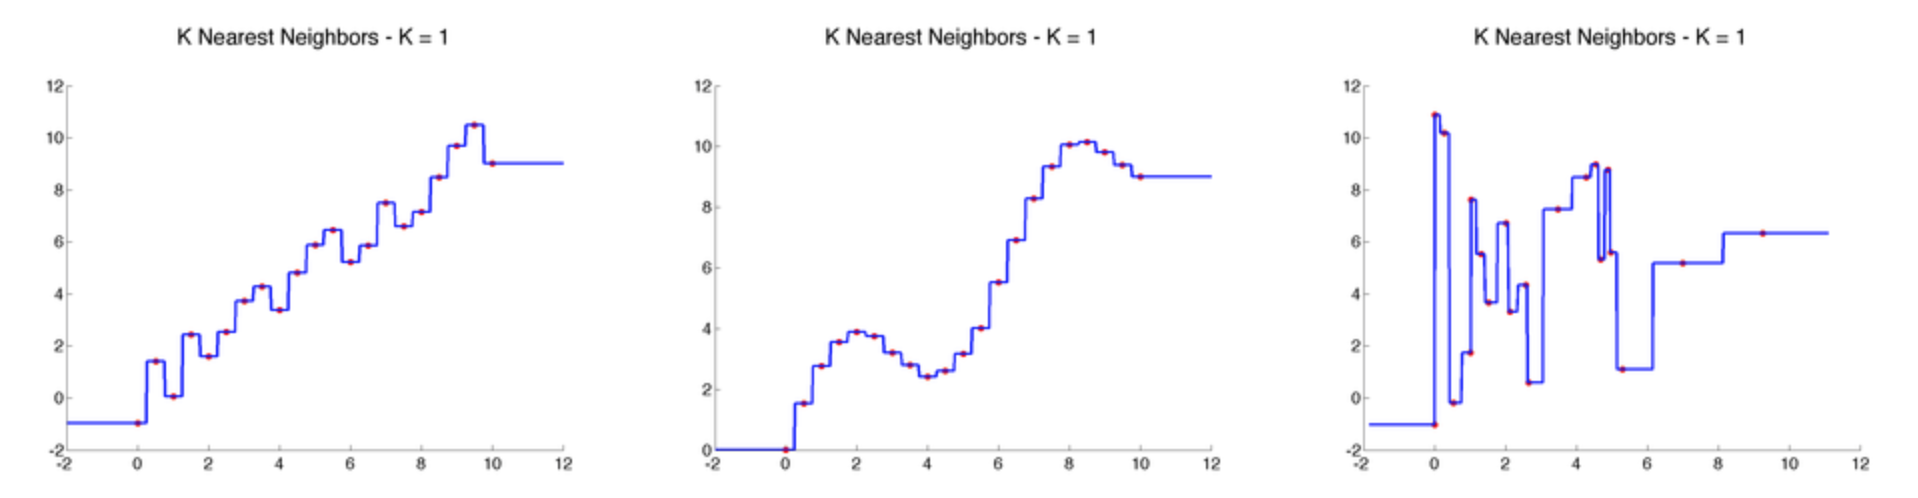
\includegraphics[width=6in]{1NN.png}
\end{figure}

Generally, we use some arbitrary distance function to define nearest neighbor. Some common choices are the $L_1$, $L_2$, or the $L_{\infty}$ norms. 

\begin{defn}
\textbf{Norm} - for all $a \in \mathbb{R}$ and all $u,v \in V$,
\begin{itemize}
\item $L_p(av) = |a|L_p(v)$
\item $L_p(u+v) \leq L_p(u) + L_p(v)$ - \emph{triangle inequality or subadditivity}
\item If $L_p(v)=0$ then v is the zero vector
\end{itemize}
\end{defn}

\begin{ex}
$L_p$ norm : $\left(\sum_{j}|x_j|^p\right)^{\frac{1}{p}}$
\end{ex}

\begin{defn}
\textbf{$L_0$ pseudo-norm} : $|x|_0$ = number of $x_j \neq 0$ 
\end{defn}

The contours of the most common distance measures are below.

\begin{figure}[H]
\centering
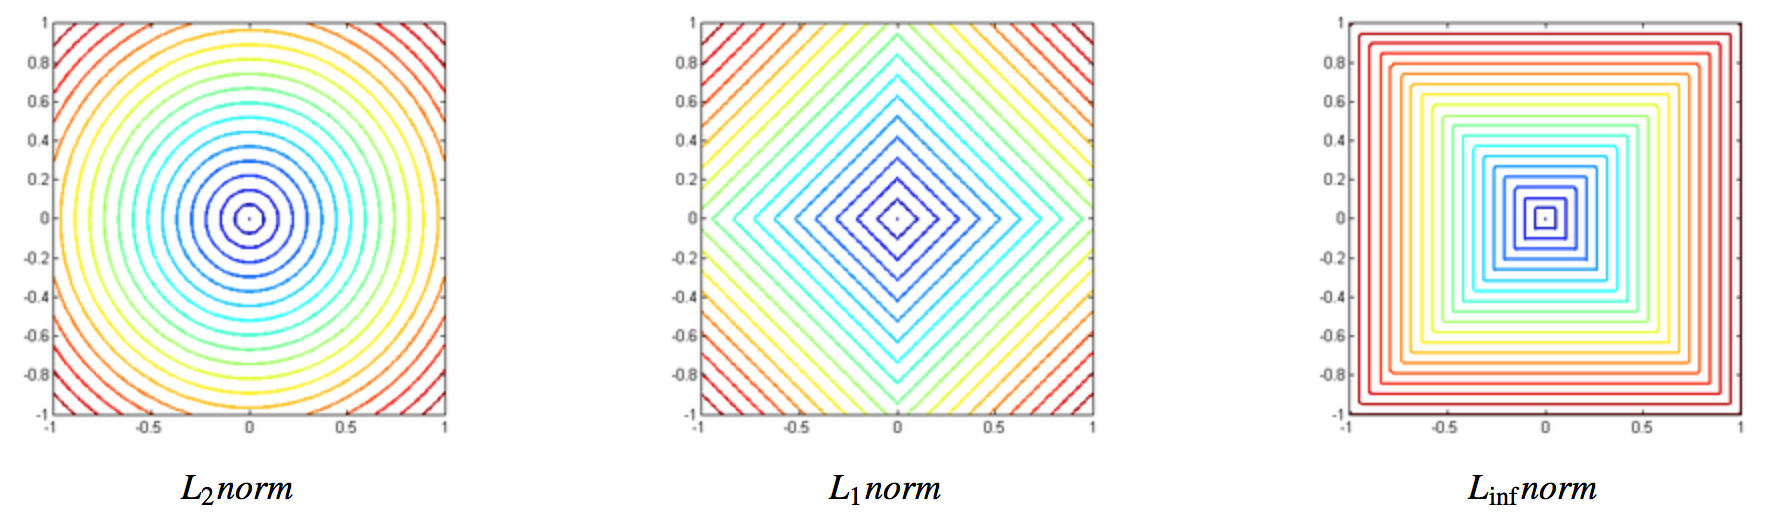
\includegraphics[width=6in]{norm_contour.png}
\end{figure}

Note that for the $L_p$ norm, p must be at least 1. $L_p$ norms with $p<1$ result in \textbf{concave} contours - NOT GOOD. So how do norms delate explicitly to distances?

\begin{equation*}
d_p(x,y) = |x-y|_p
\end{equation*}

Note that norms are \textbf{SCALE-INVARIANT}. Thus, if $x$ is a vector of non-negative terms, then 
\begin{align*}
\sum_i x_i \hspace{0.5in} \text{and} \hspace{0.5in} \sum_i ix_i
\end{align*}

are both norms. \\

1-Nearest Neighbor is one of the simplest examples of a \textbf{non-parametric} method (ie. model structure determined by the training data). Non-parametric models are much more flexible and expressive than parametric models, and thus \textbf{overfitting} can be a big concern. One nice property of NP models is that since the complexity increases as the data increases, with enough data, NP models can model nearly anything and achieve close to zero bias for any distribution (ie. consistent..sort of). A huge problem with this, however, is that for any finite sample size there will likely be huge variance (ie. overfitting). \\

One way to reduce the variance is local averaging : instead of just one neighbor, find K and average their predictions. 

\begin{verbatim}
K-Nearest Neighbors Algorithm
  1. Given training data D={x_i,y_i}, distance function d(.,.), and input x
  2. Find {j_1,...,j_K} closest examples wrt d(x,.)
      a. (Regression) if y \in \mathbb{R}, return average of y_{j_k}
      b. (Classification) if y is 1 or -1, return majority
\end{verbatim}

\begin{figure}[H]
\centering
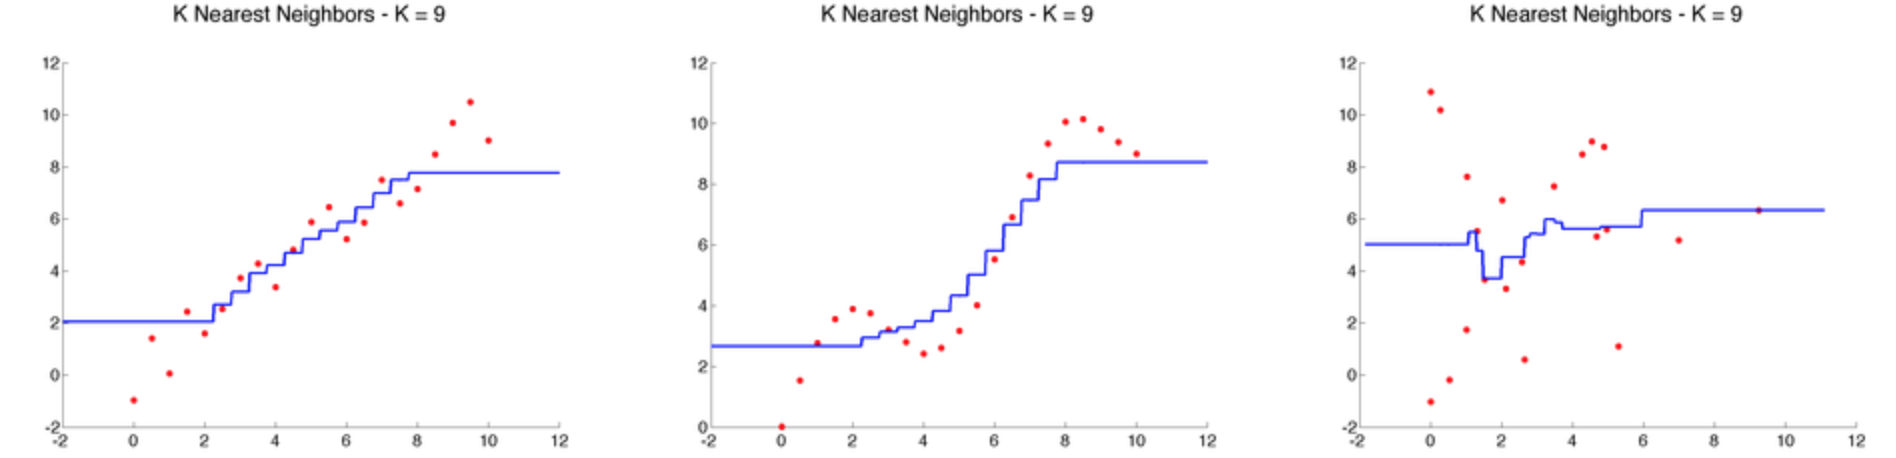
\includegraphics[width=6in]{9NN.png}
\caption{9 nearest neighbors - smoother prediction but edges still sketchy}
\end{figure}

\subsection{Kernel Regression}

Two main shortcomings of K-NN method:
\begin{enumerate}
\item All neighbors receive equal weight
\item Number of neighbors chosen globally
\end{enumerate}

Kernel regression address these issues by \emph{using all neighbors} but with different weights (ie. closer neighbors receiving higher weights and vice versa). Weighting function is a \textbf{kernel} and it measures similarity (as opposed to distance) between examples. Can convert from a distance d(.,.) to kernel K(.,.) easily - most common way is via Gaussian kernel (ignoring normalizing constants):

\begin{equation*}
K(x,x_i) = \exp\left(\frac{-d^2(x,x_i)}{h}\right)
\end{equation*}

Kernel Regression/Classification Algorithm
\begin{enumerate}
\item Given training data $D={x_i,y_i}$, Kernel function K(.,.), and input x
\begin{itemize}
\item (Regression) if $y \in \mathbb{R}$, return weighted average: $\sum_i y_i \frac{K(x,x_i)}{\sum_j K(x,x_j)}$
\item (Classification) if $y \in \pm 1$, return weighted majority: $\mbox{sgn}\left(\sum_i y_iK(x,x_i)\right)$
\end{itemize}
\end{enumerate}

One of the keys kernel regression is $h$, the \textbf{bandwidth}, which determines how quickly the influence of neighbors falls off with distance. The following shows the effect of increasing levels of $h$. 

\begin{figure}[H]
\centering
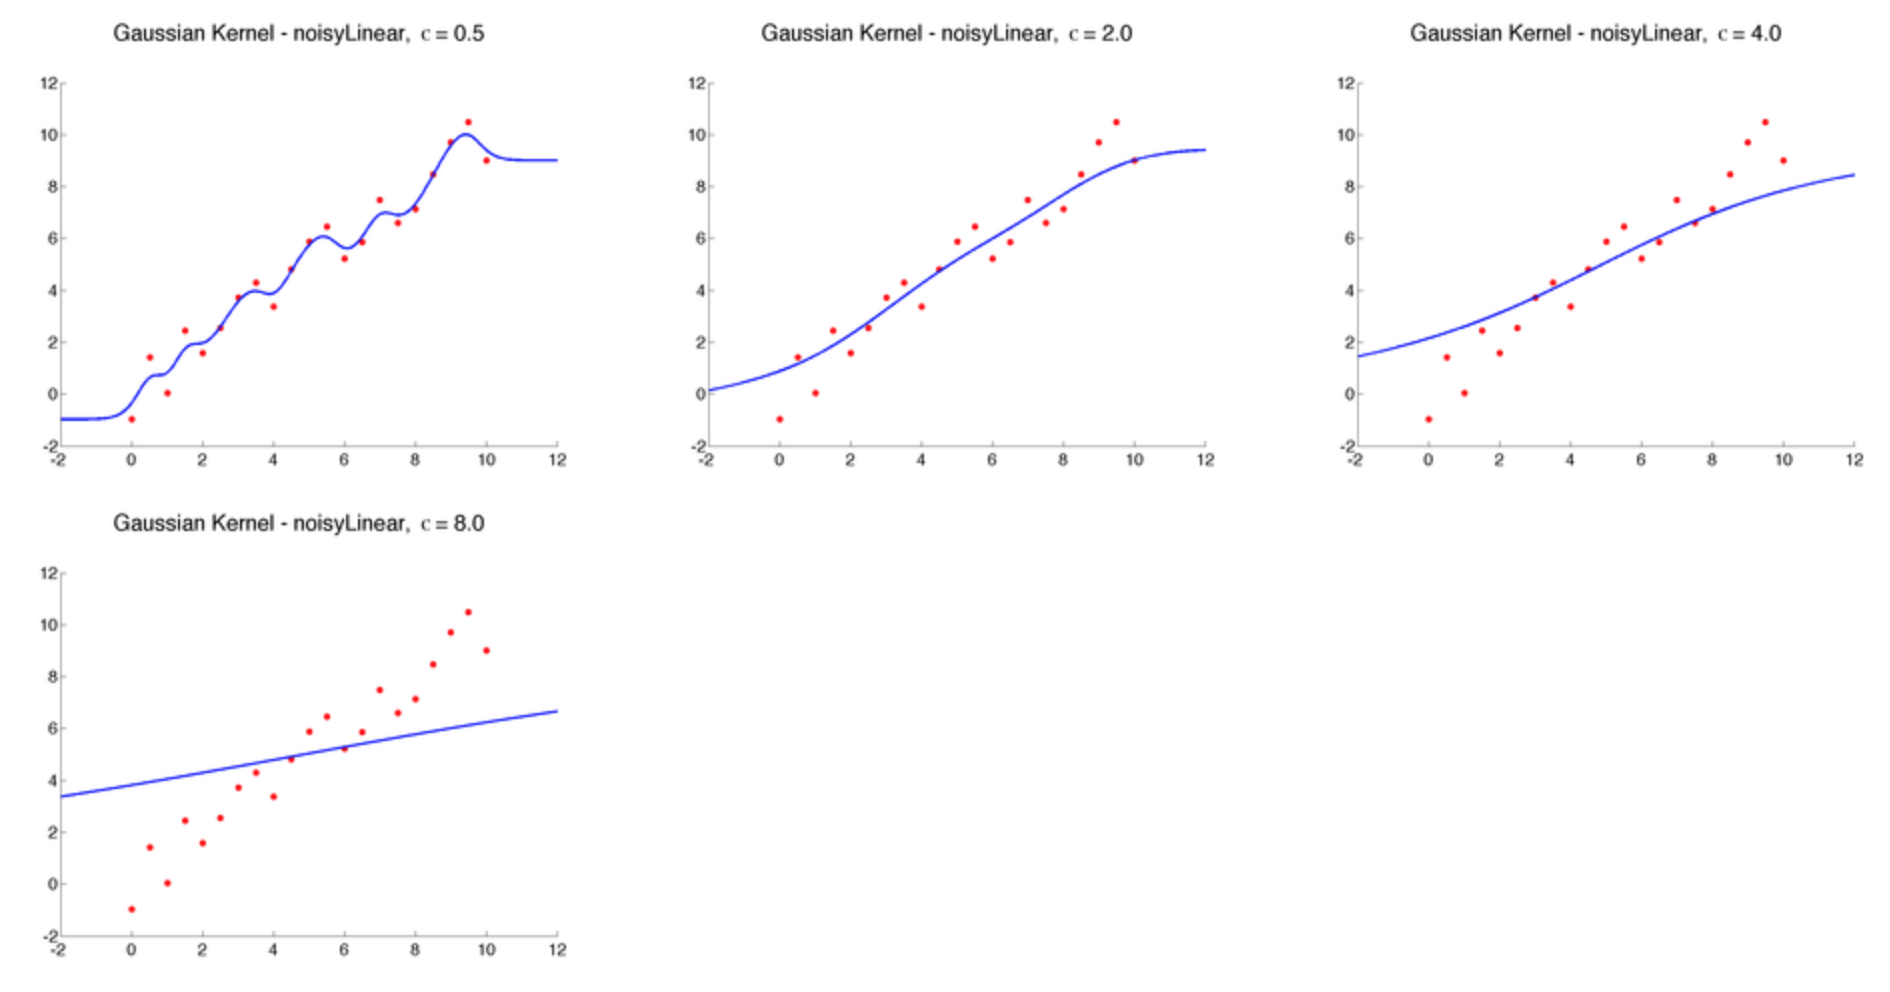
\includegraphics[width=6in]{kernel_reg.png}
\end{figure}

As $h \rightarrow \infty$, all the neighbors weight the same and the prediction is the global average. \\
As $h \rightarrow 0$, prediction tends to 1-NN. \\
Clearly choosing the ``right" $h$ is very important - in practice, usually use \textbf{cross-validation} to pick.

\section{Decision Trees}

\begin{itemize}
\item Gives nice interpretable output but each split uses exponentially less data (observations)
\item How do we decide which features to split on? How to define importance? Need definition of information
\end{itemize}

\subsection{Entropy}
Suppose X can have one of $m$ values, $V_1,\ldots,V_m$, with $P(X=V_i)=p_i$. Entropy is the smallest possible number of bits, on average, per symbol, needed to transmit a stream of symbols drawn from X's distribution. 

\begin{defn}
Entropy : $H(X) = -\sum_{j=1}^m p_j \log_2 p_j$
\end{defn}

\begin{itemize}
\item High entropy : X is from uniform (boring) distribution. Values sampled from it would be all over the place.
\item Low entropy : X is from varied (valleys and peaks) distribution. Values sampled from it would be more predictable (from the peaks).
\end{itemize}

\textbf{Entropy} is the expected value of the information content (surprise) of the message $\log_2 p_j$. Range of entropy is from 0 to $\infty$. 

\begin{ex}
\begin{enumerate}
\item If an event is certain, entropy is 0
\item If two events are equally likely, entropy is 1 $(-\left(-0.5 * \log(0.5) + -0.5 * \log(0.5)\right)$
\end{enumerate}
\end{ex}

\begin{defn}
Specific Conditional Entropy : $H(Y|X=v)$, the entropy of Y among only those records in which X has value v.
\end{defn}

\begin{figure}[H]
\centering
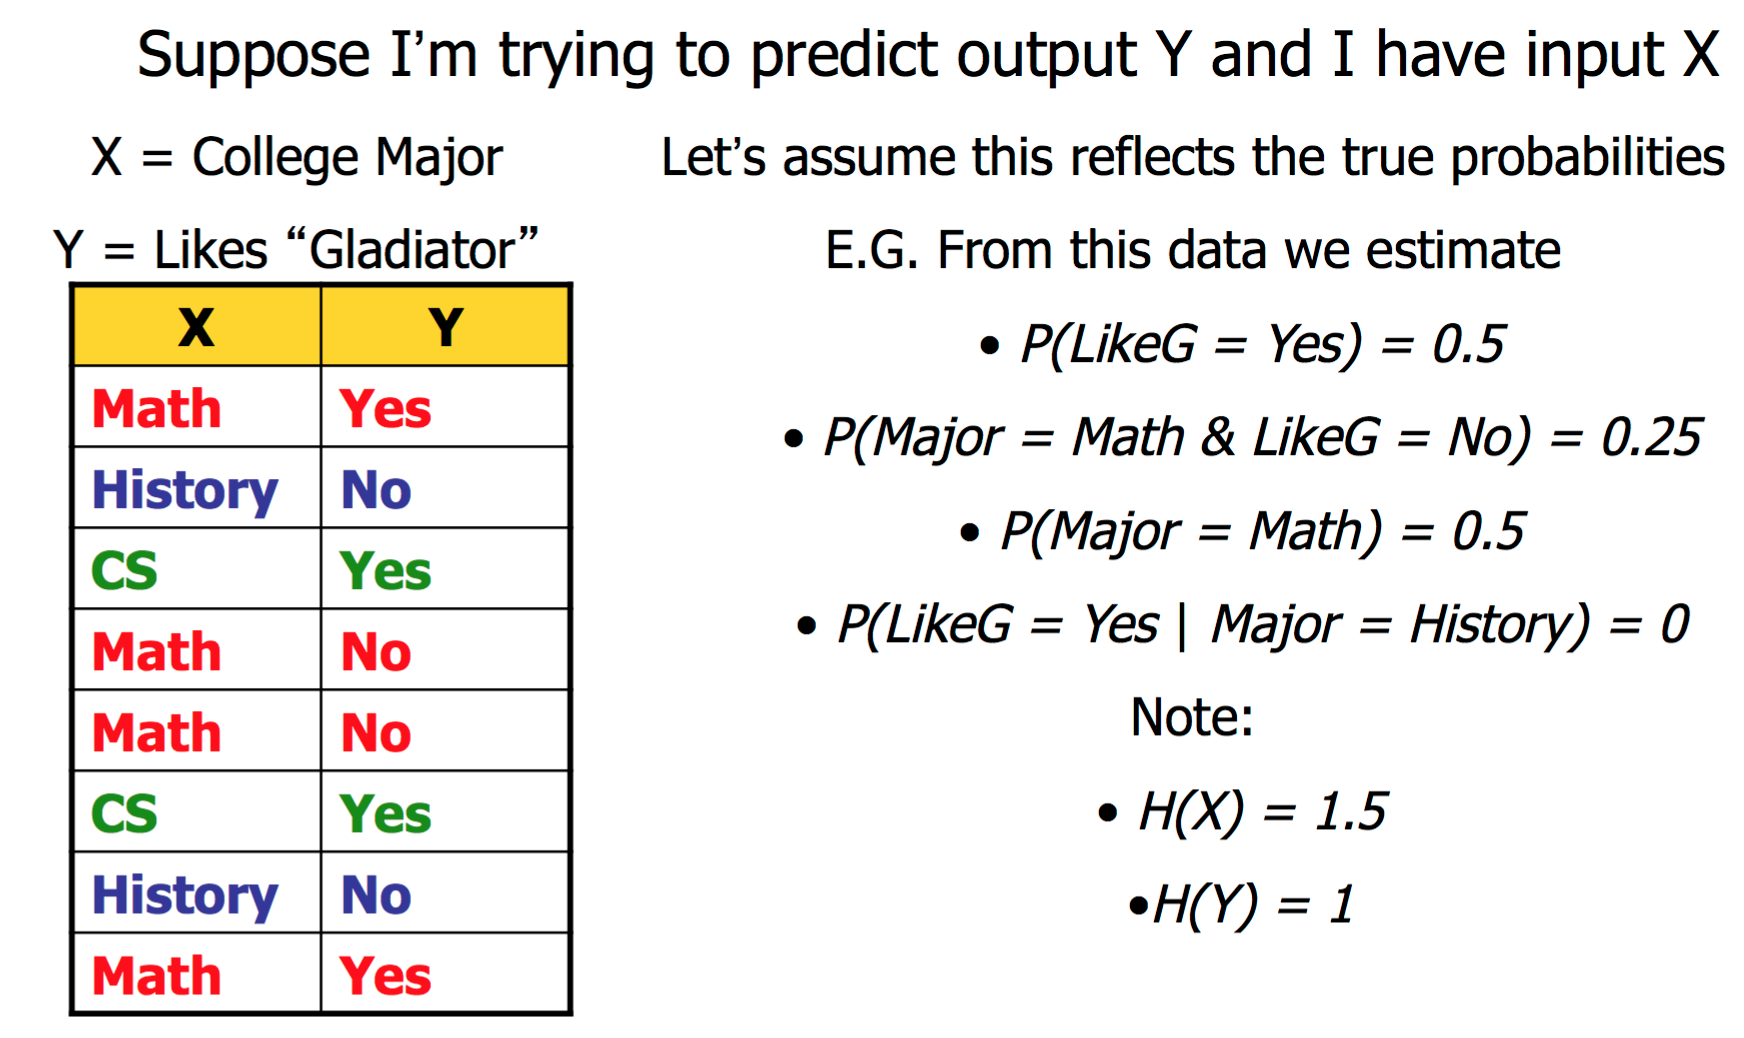
\includegraphics[width=6in]{cond_ent_ex.png}
\end{figure}

\begin{defn}
Conditional Entropy : $H(Y|X)=\sum_j P(X=v_j)H(Y|X=v_j)$, the average specific conditional entropy of Y 
\end{defn}


\begin{figure}[H]
\centering
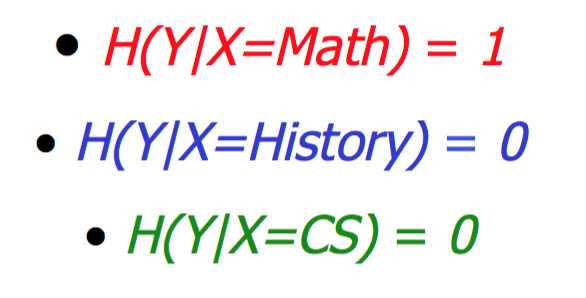
\includegraphics[width=1.5in]{specific_condent.png}
\end{figure}

\begin{defn}
Information Gain : $IG(Y|X) = H(Y)-H(Y|X)$, how many bits on average would it save me in transmitting Y if both ends of the line knew X? 
\end{defn}

\begin{ex}
Suppose, \\
$H(Y)=1, H(Y|X)=0.5$. Then $IG(Y|X) = 1-0.5=0.5$, and knowing X gives gain of 0.5 information (unit is bits). 
\end{ex}

Note: range of IG is from 0 to $\infty$. If Y and X are independet, then $IG=0$. \\
In general, features with more options (more categories) have more possible information gain than binary features. \\
\\
\textbf{Key to Decision Trees}: How do we prevent overfitting? How we know when to stop splitting?! Number of leaves grows exponentially


\section{MLE}

Self-explanatory. 

\subsection{Learning Guarantees}

The following bound will be useful (based on Hoeffding inequality): 

\begin{thm}
$P(|\hat{\theta}_{MLE}-\theta| \geq \epsilon) \leq 2e^{-2n\epsilon^2}$
\end{thm}

In other words, MLE deviates from true parameter exponentially with $n$. 

\section{MAP (maximum a posteriori)}

Bayes rule gives 

\begin{equation*}
P(\theta|D) = \frac{P(D|\theta)P(\theta)}{P(D)}
\end{equation*}

\begin{defn}
$\hat{\theta}_{MAP} = \mbox{arg max}_{\theta} P(\theta|D) = \mbox{arg max}_{\theta} \log(P(D|\theta)) + \log(P(\theta)) $
\end{defn}

Note: the $\log(P(\theta))$ acts as a regularizer for the log likelihood for MAP estimation. \\
Note: as $n \rightarrow \infty$, the prior's effect vanishes and we recover the MLE.\\
Note: MAP is the simplest Bayesian approach to parameter estimation - sets estimate equal to mode of posterior distribution $P(\theta|D)$. There is more information in the posterior such as the mean and variance of the distribution. 


\section{Regression}


\section{Classification}

If we had binary data (0's and 1's), we could fit linear regression and just predict everything $>0.5$ to be 1 and everything $<0.5$ to 0. We \textbf{CAN} fit linear regression to binary data, but this is bad!! This gives probabilities below 0 and above 1!! \\
\\
Make a transformation! Most common one is \textbf{logit} function:
\begin{equation*}
f(s) = \frac{1}{1+e^{-s}}
\end{equation*}

\subsection{Logistic Regression}

Thus we obtain something like (for Y=1 and Y=-1)
\begin{align*}
P(Y=1|x,w) &= \frac{1}{1+\exp(-w^Tx)} = \frac{1}{1+\exp(-yw^Tx)} \\
P(Y=-1|x,w) &= 1-P(Y=1|x,w) = \frac{\exp(-w^Tx)}{1+\exp(-w^Tx)} = \frac{1}{1+\exp(-yw^Tx)} \\
\end{align*}

Since log-likelihood for logistic regression is convex, can solve using \textbf{gradient ascent/descent}! \\
\\
Can also do the same with multinomial outcomes!
\begin{align*}
P(Y=k|x,w) = \frac{\exp(w_k^T x)}{1+\sum_{k'=1}^{K-1} \exp(w_{k'}^T x)} \hspace{0.3in} k=1,\ldots,K
\end{align*}

\subsection{Naive Bayes}

Naive Bayes classifier is an example of a \textbf{generative} model : we model $P(x,y)=P(y)P(x|y)$ where
\begin{itemize}
\item $P(y)$ : class prior
\item $P(x|y)$ : class model
\end{itemize}

We estimate them separately as $\hat{P(y)}$ and $\hat{P(x|y)}$. Note: the class prior is different than the parameter prior classic Bayesian analysis. We then use our estimates to output a classifier using Bayes rules:

\begin{align*}
h(x) = \text{argmax}_y \hat{P(y|x)}  = \text{argmax}_y \frac{\hat{P(y)}\hat{P(x|y)}}{\sum_y \hat{P(y)}\hat{P(x|y)}} \propto \text{argmax}_y \hat{P(y)}\hat{P(x|y)}
\end{align*}

\text{In English}: Classify a new instance $x$ based on a tuple of attribute values $x=(x_1,\ldots,x_n)$ into one of the classes $y_j \in Y$. \\
\\

\textbf{Estimating $P(y)$} : Can be estimated from the frequency of classes in the training examples\\
\\
\textbf{Estimating $P(x|y)$} : The \emph{Naive Bayes assumption} is that $P(x|y) = \prod_i \hat{P(x_i|y)}$ (Conditional independence) \\
\\

If we assume both $Y$ and $X$ are discrete, can do (MLE estimation)
\begin{align*}
\hat{P(y)} = \frac{N(y=y_j)}{N} \hspace{0.5in} \hat{P(x_i|y)} = \frac{N(x_i=x_j,y=y_j)}{N(y=y_j)}
\end{align*}

Note: If $Y$ and/or $X$ are continuous, we can pick some model for the distribution (ie. Gaussian). \\
\\

Problem with MLE though is that if we see no training examples for some class, we have 0 probabilities! To deal with this, we can smooth the probabilities to avoid overfitting. 
\begin{align*}
\hat{P(x_i|y)} = \frac{N(x_i=x_j,y=y_j)+mP_{i,k}}{N(y=y_j)+m}
\end{align*}

This is sort of like \textbf{empirical bayes} where our prior includes information on probabilities in the entire sample?  \\
\\
Note for implementation: DO NOT MULTIPLY PROBABILITIES. THIS LEADS TO UNDERFLOW. INSTEAD ADD LOG PROBABILITIES.






\end{document}
